\chapter{Contexte general du projet :}
\section{Presentation du centre :}
Le Code 212 est un centre de formation et de certification dans les metiers du digital, lance dans le cadre du Plan d'Acceleration de la Croissance et de la Transformation de l'economie (PACTE) ESRI-2030 au Maroc. Ce programme vise à repondre aux enjeux actuels et futurs lies à l'emergence des technologies numeriques en offrant des filières specifiques et des formations certifiantes. L'objectif est de renforcer les competences et les qualifications dans le secteur numerique, contribuant ainsi à l'atteinte des objectifs de developpement du pays, notamment celui de faire passer la part du secteur numerique à 5% du PIB d'ici 2035.

Le principal objectif du Centre Code 212 est de former une nouvelle generation de professionnels qualifies dans le domaine du numerique afin de repondre aux besoins croissants du marche de l'emploi dans ce secteur en plein essor. En offrant des formations specialisees et des certifications reconnues, le centre vise à fournir aux apprenants les competences et les connaissances necessaires pour reussir dans des domaines tels que le developpement web, la cybersecurite, l'analyse de donnees, le marketing digital et bien d'autres. En outre, le centre s'engage à promouvoir l'innovation et l'entrepreneuriat en encourageant les initiatives creatives et en offrant un environnement propice à l'emergence de projets novateurs dans le domaine du digital.

\subsection{Fiche du centre Code 212}

\begin{tabularx}{\textwidth}{|l|X|}
\hline
\textbf{Nom du Centre} & Code 212 \\
\hline
\textbf{Domaine d'Activite} & Formation et certification dans les metiers du digital \\
\hline
\textbf{Programme} & Plan d'Acceleration de la Croissance et de la Transformation de l'economie (PACTE) ESRI-2030 \\
\hline
\textbf{Localisation} & Agadir Maroc \\
\hline
\textbf{Objectif} & Renforcer les competences et les qualifications dans le secteur numerique \\
\hline
\textbf{Domaines de Formation} & 
\begin{tabular}{@{}l@{}}
- Developpement web \\
- Cybersecurite \\
- Analyse de donnees \\
- Marketing digital \\
- et bien d'autres
\end{tabular} \\
\hline
\textbf{Engagement} & 
\begin{tabular}{@{}l@{}}
- Promouvoir l'innovation \\
- Encourager l'entrepreneuriat \\
- Offrir un environnement propice aux projets novateurs
\end{tabular} \\
\hline
\end{tabularx}


\subsection{Centre Code212}
\begin{figure}[H]
\centering
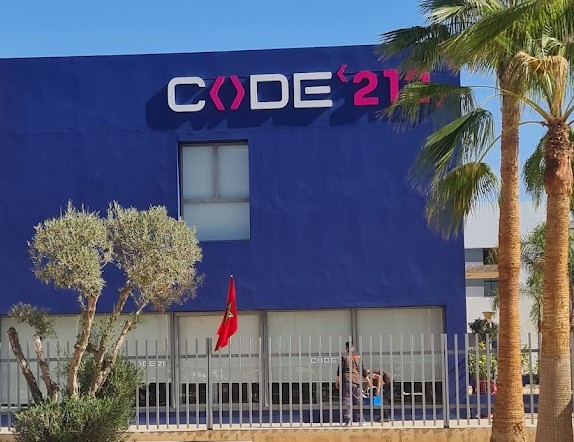
\includegraphics[height=10cm , width=\textwidth]{assets/images/code.jpg}
\caption{Centre Code 212 Agadir}
\label{fig:imagecentre}
\end{figure}

\begin{figure}[H]
\centering
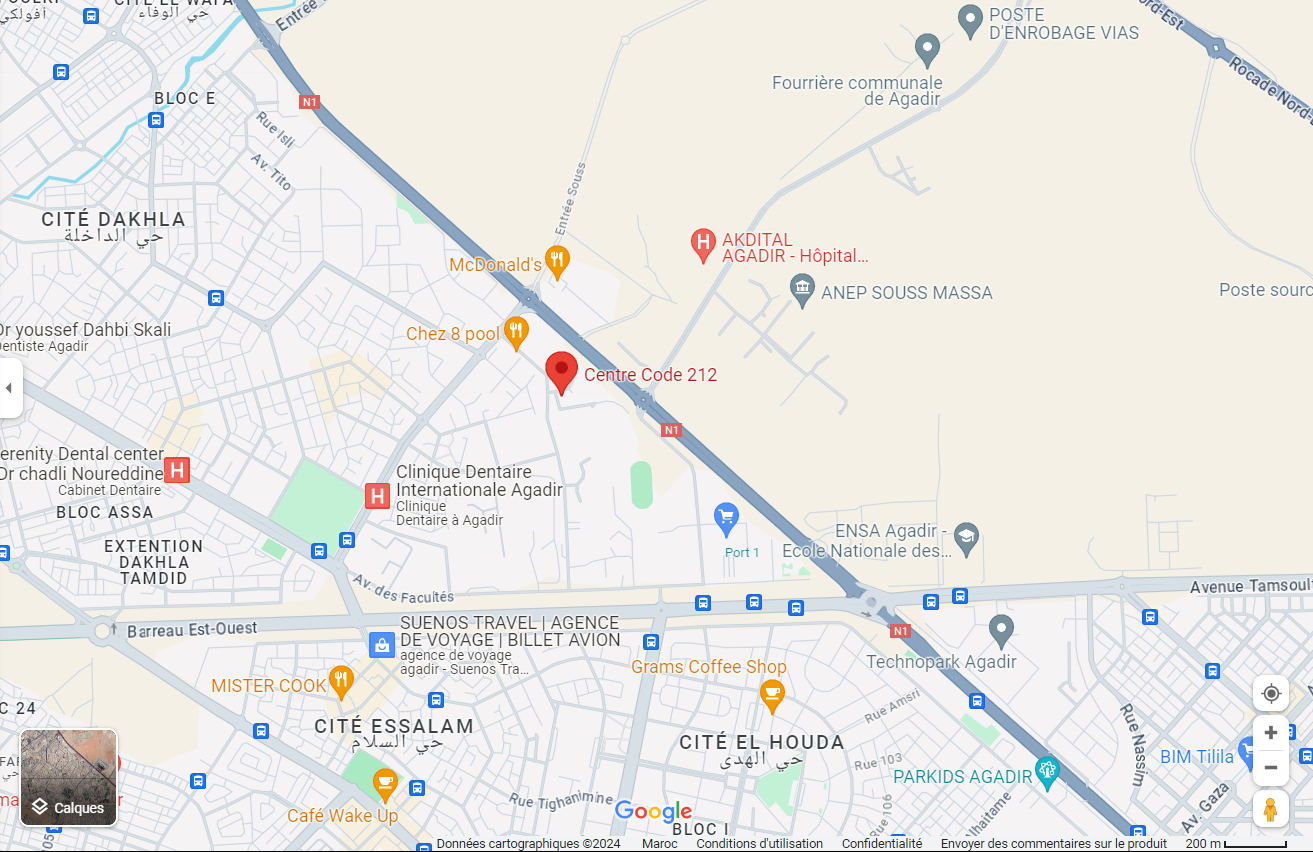
\includegraphics[height=10cm , width=\textwidth]{assets/images/maps.png}
\caption{Localisation du centre}
\label{fig:localisationcentre}
\end{figure}

\subsection{Domaines d'activites et expertise :}

Le centre Code 212 d'Agadir developpe son expertise autour de plusieurs axes strategiques, visant à repondre aux exigences du marche numerique moderne et aux besoins de transformation digitale du Maroc.

\subsubsection{Education et Pedagogie innovante :}

\paragraph{Methodologie d'apprentissage :}
L'education au sein du centre Code 212 repose sur une approche pedagogique revolutionnaire qui rompt avec les methodes traditionnelles d'enseignement. Cette methode, connue sous le nom de \textbf{peer-to-peer learning}, place l'apprenant au centre du processus educatif et favorise :

\begin{itemize}
    \item \textbf{Apprentissage collaboratif} : Les etudiants travaillent en equipes pour resoudre des projets concrets, simulant ainsi l'environnement professionnel reel
    \item \textbf{Autonomie pedagogique} : Absence de cours magistraux traditionnels, encourageant l'auto-apprentissage et la recherche personnelle
    \item \textbf{Mentorat mutuel} : Les etudiants avances accompagnent les debutants, creant une dynamique d'entraide et de partage de connaissances
    \item \textbf{Evaluation par les pairs} : Systeme d'evaluation base sur la correction mutuelle des projets
\end{itemize}

\paragraph{Infrastructure technologique :}
Le centre dispose d'equipements de pointe incluant :
\begin{itemize}
    \item Laboratoires informatiques equipes de stations de travail haute performance
    \item Plateforme d'apprentissage en ligne personnalisee
    \item Environnements de developpement integres (IDE) professionnels
    \item Acces aux technologies cloud et aux outils de developpement modernes
\end{itemize}

\subsubsection{Renforcement des competences et employabilite :}

\paragraph{Programmes de formation specialises :}
Code 212 Agadir propose un curriculum adapte aux exigences du marche du travail numerique, structuré autour de plusieurs piliers :

\begin{enumerate}
    \item \textbf{Socle technique fondamental :}
    \begin{itemize}
        \item Algorithmique et structures de donnees
        \item Programmation orientee objet
        \item Bases de donnees et gestion de l'information
        \item Architectures logicielles et design patterns
    \end{itemize}
    
    \item \textbf{Technologies emergentes :}
    \begin{itemize}
        \item Intelligence artificielle et machine learning
        \item Developpement web full-stack (Frontend/Backend)
        \item Applications mobiles natives et cross-platform
        \item Cloud computing et DevOps
        \item Cybersecurite et protection des donnees
    \end{itemize}
    
    \item \textbf{Competences transversales :}
    \begin{itemize}
        \item Gestion de projets agiles (Scrum, Kanban)
        \item Travail en equipe et communication
        \item Entrepreneuriat et innovation
        \item Veille technologique et apprentissage continu
    \end{itemize}
\end{enumerate}

\paragraph{Partenariats et insertion professionnelle :}
Le centre maintient des relations etroites avec l'ecosysteme economique local et national :
\begin{itemize}
    \item \textbf{Partenariats entreprises} : Collaboration avec des startups et des multinationales pour des projets reels
    \item \textbf{Stages professionnels} : Programme de stages obligatoires en entreprise
    \item \textbf{Job dating} : Organisation regulière d'evenements de recrutement
    \item \textbf{Incubation} : Accompagnement des projets entrepreneuriaux des etudiants
\end{itemize}

\paragraph{Suivi et accompagnement :}
\begin{itemize}
    \item Coaching personnalise pour chaque etudiant
    \item Suivi post-formation pendant 12 mois
    \item Reseau alumni actif
    \item Formation continue et certification professionnelle
\end{itemize}
